\documentclass{beamer}
\usepackage{graphicx}
\usepackage{tikz}
\usepackage{pgfplots}

\pgfplotsset{compat=newest}

\usetheme{Madrid}

\title{Self-Balancing Bike}

\titlegraphic{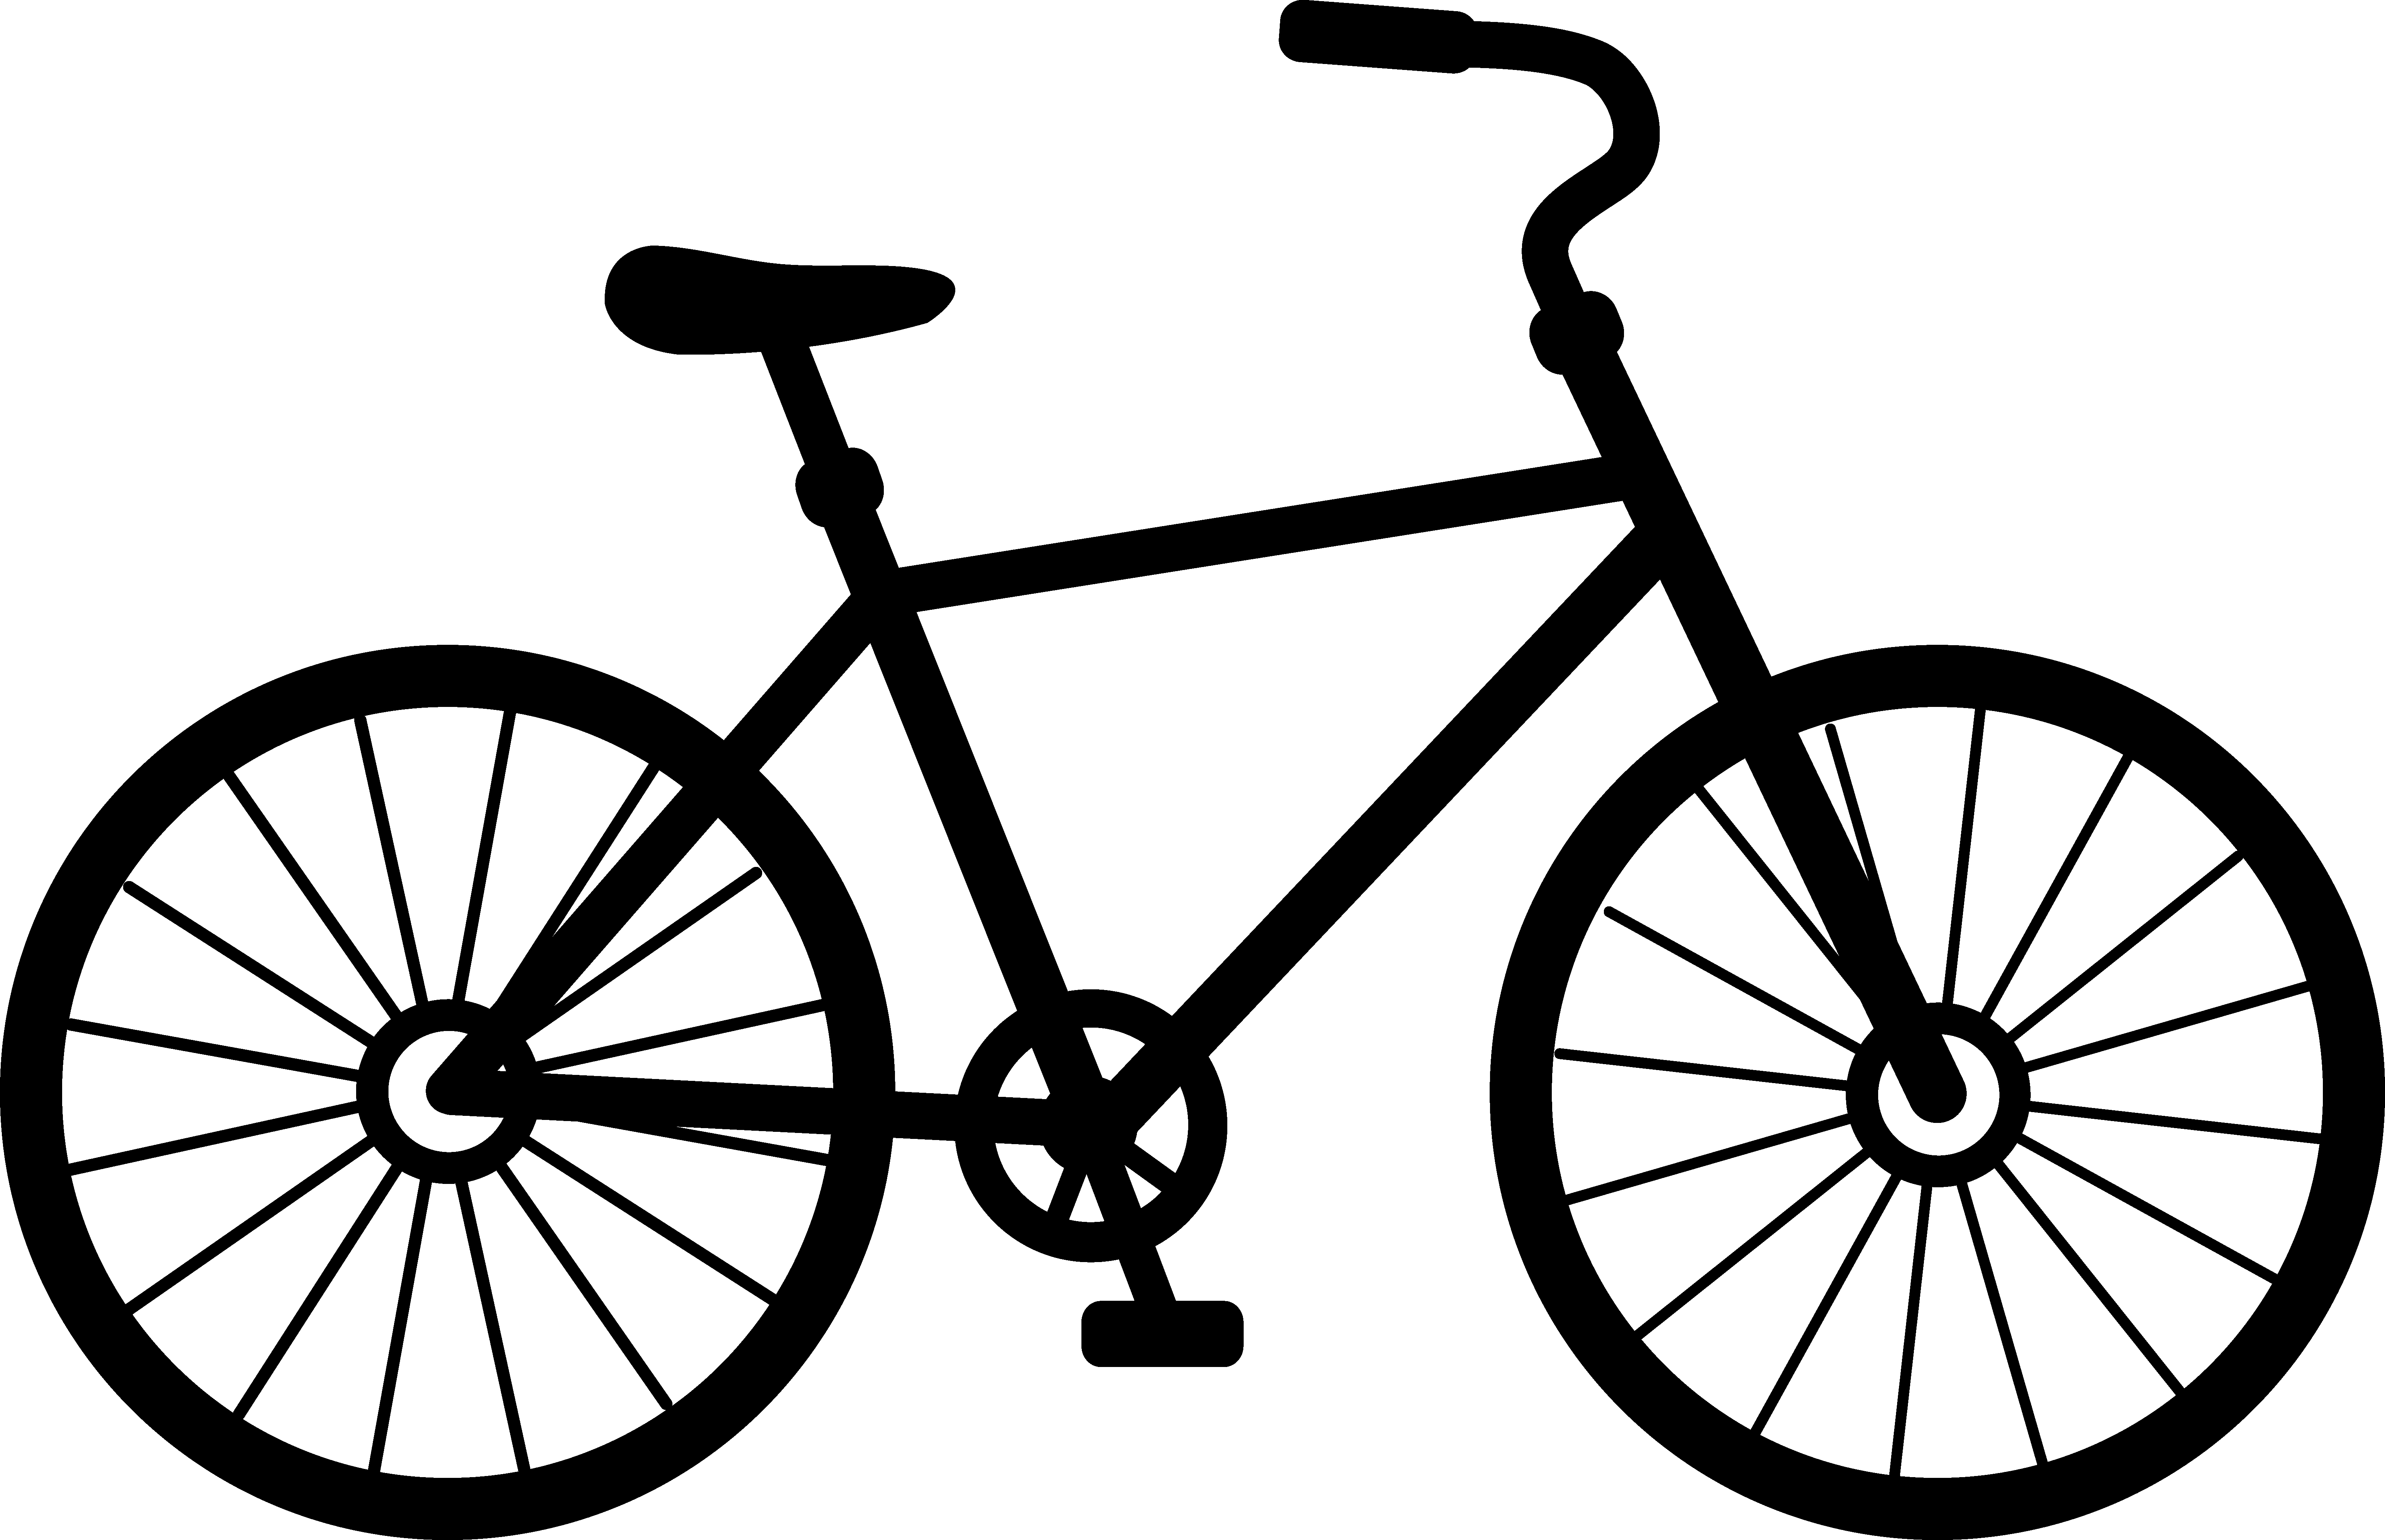
\includegraphics[scale=0.075]{Bike.png}}

\author{Philip Salmony, Wolfson College}

\date{November 22, 2018}

\begin{document}

\begin{frame}
  \titlepage
\end{frame}


\section{First Main Section}

\subsection{First Subsection}

\begin{frame}{Background and Context}

  \begin{itemize}
  \setlength\itemsep{0.5em}
  \item {Bicycle stability and equations of motion studied for well over 100 years.}
  \item {Still misconceptions about why a bike is self-stable. Typical explanation: gyroscopic effects of wheels.}
  \item {Similar to inverted pendulum but with more degrees of freedom.}
  \item {Under-actuated system: Rider-less, therefore can only actuate rear wheel and handlebars.}
  \end{itemize}
    
\end{frame}

\subsection{Aims and Significance}

\begin{frame}{Aims and Significance}

	\begin{itemize}
	\setlength\itemsep{0.75em}
		\item {How does a human stabilise a bicycle and can we replicate this behaviour with motors?}
		\item {What makes a bicycle more or less stable (such as changes in geometry, mass distributions, wheel size,
etc.)}?
		\item {Would there be a benefit in having an 'assisted' bicycle for certain people and situations? (see \textit{Honda Self-Balancing Bike})}
		\item {Can we design a control algorithm that stabilises a bicycle in all situations (speeds, extra weight, etc.)?}
		\item {Generally, an interesting but very difficult control problem.}
  		\end{itemize}
  
\end{frame}

\begin{frame}{Honda Self-Balancing Bike}

	\centering
	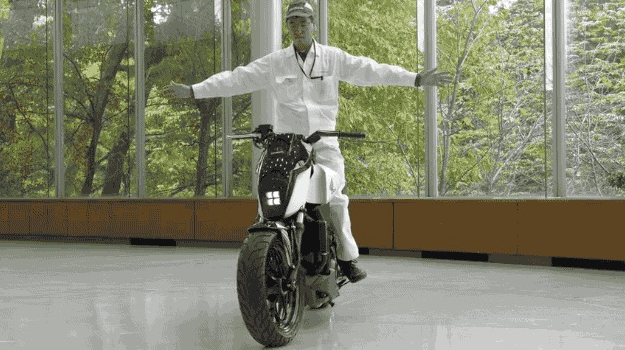
\includegraphics[scale=0.6]{Honda}
	October 2017 - fairly recent!
	
\end{frame}

\subsection{Progress}

\begin{frame}{Progress - Modelling}
 
  \begin{itemize}
  
  	\setlength\itemsep{0.5em}
  	\item {\textbf{Linear and non-linear bicycle models} for simulation}
  	
  	\begin{itemize}
  		\item Many, very complex and coupled non-linear, differential equations.
  		\item Commonly used fourth-order linearised model, dependent on forward speed.
  	\end{itemize}
  	
  	\item {\textbf{Stability investigation}}
  	\begin{itemize}
  		\item Common theories: Gyroscopic effects, trail of fork?
  		\item Mass distribution? Dependence on forward speed?
  	\end{itemize}
  	
	\item {Developed \textbf{simulations} in Unity and MatLAB/Simulink}
	
	\begin{itemize}
		\item Basis for testing control algorithms, including robustness tests.
		\item Visualisation of bicycle dynamics.
		\item Useful for discrete controller implementation later on.
	\end{itemize}		
	
  \end{itemize}
    
\end{frame}

\begin{frame}{Progress - Simulator}

  \centering
  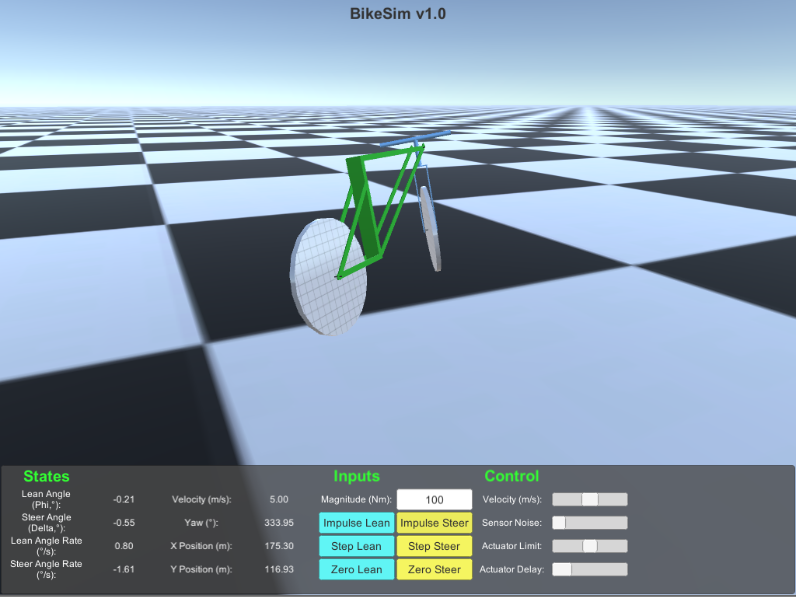
\includegraphics[scale=0.475]{BikeSim}

\end{frame}

\begin{frame}{Progress - Controller Design}
 
  \begin{itemize}
  
  	\setlength\itemsep{0.5em}
 
  	\item {Investigated \textbf{classical SISO and MIMO controller design}}

	\item{Developed \textbf{LEGO Mindstorms prototype} for preliminary testing of control algorithms}
	
  	\item{Started looking into advanced \textbf{non-linear control}}
  	
  	\begin{itemize}
  		\item{Virtual Model Control: connecting \textit{virtual} springs and dashpots to real-world model.}
  		\item{Energy-Balancing Control: can we shape the energy function of the closed-loop system to have a new, different minimum?}
  	\end{itemize}
  
  \end{itemize}
    
\end{frame}

\subsection{Findings}

\begin{frame}{Findings So Far (Excerpt)}

	\begin{itemize}
	
		\setlength\itemsep{0.5em}
	
		\item Non-linear model far too hard to interpret intuitively, also difficult for controller design.
		\item Stability \textit{strongly} dependent on forward speed.
		\item Difficult system to control: RHP zeros and poles.
		\item In theory, classical linear control (PD), as well as multi-variable control (LQR) can stabilise a rider-less bicycle.	
	
	\end{itemize}
	
	\centering
	\begin{figure}[H]
	\scalebox{0.6}{
	\begin{tikzpicture}
		\begin{axis}
			[xlabel=Forward Speed $v$,
			 ylabel=Real Part of Eigenvalue $\lambda$,
			 xmin=0,xmax=6,
			 ymin=-10,ymax=5]
			\addplot[mark=none] table[x=v,y=a, col sep=comma] {StabilityVsForwardSpeed.csv};
			\addplot[mark=none] table[x=v,y=b, col sep=comma] {StabilityVsForwardSpeed.csv};
			\addplot[mark=none] table[x=v,y=c, col sep=comma] {StabilityVsForwardSpeed.csv};
			\addplot[mark=none] table[x=v,y=d, col sep=comma] {StabilityVsForwardSpeed.csv};
			
			\draw [dashed, thin] (0,0) -- (6,0);
			\draw [dotted, thin] (3,-10) -- (3,5);
			\draw [dotted, thin] (4.8,-10) -- (4.8,5);
		\end{axis}
	\end{tikzpicture}
	}
\end{figure}

\end{frame}

\subsection{Plans}

\begin{frame}{Plans}

  \begin{itemize}
  	\setlength\itemsep{1em}
  	
	\item{\textbf{Michaelmas}}  	
	\begin{itemize}
		\item{Finalise LEGO prototype.}
		\item{Further investigate non-linear control.}
	\end{itemize}	  	
  	
	\item{\textbf{Lent}}
	\begin{itemize}
		\item{Robust control: e.g. $H_\infty$ loop shaping.}
		\item{If LEGO prototype is self-stable, move on to \textit{full scale bike}!}
	\end{itemize}		
  
	\item{\textbf{General}}
	\begin{itemize}
		\item{Bike very hard to control at low speeds, can we use extra actuators?}
	\end{itemize}  
  
  \end{itemize}

\end{frame}

\end{document}